\documentclass[10pt,conference,compsocconf]{IEEEtran}

%\usepackage{times}
%\usepackage{balance}
\usepackage{url, amsmath, amssymb}
\usepackage{graphicx}    % For figure environment
\usepackage{textcomp}
\usepackage{amsfonts}
\usepackage[ruled,vlined]{algorithm2e}

\usepackage[hidelinks,bookmarksnumbered,unicode]{hyperref} % Enables cross linking in the electronic document version. This package has to be included second to last.
\usepackage[noabbrev,nameinlink]{cleveref}
\usepackage{balance}
\usepackage{nag}       % Issues warnings when best practices in writing LaTeX documents are violated.
\usepackage{booktabs}
\usepackage{amsmath}   % Improves the typesettings of tables.


\newcommand{\spacing}{\hspace{1cm}}
\begin{document}
    \title{Collaborative Filtering}

    \author{
    Rafael Sterzinger \spacing Patrik Okanovic \spacing Fatjon Zogaj \spacing Filip Batur Stipic\\
    Group: Terminators\\
    Department of Computer Science, ETH Zurich, Switzerland
    }

    \maketitle

    \begin{abstract}
    Collaborative Filtering methods have become widely used in a variety of areas. In this work we consider several neural-based and standard matrix factorization methods, focusing on Bayesian Factorization Machines. We propose adding additional features. We propose upgrading Bayesian Factorization Machines with additional features.

    \end{abstract}


    \section{Introduction}

    The goal of recommender systems is to design a model which is capable of estimating a user's preference on some kind of items e.g. in our case movies.
    This is usually done by means of collaborative filtering, a standard computational method that attempts to solve this problem by leveraging the similarities between users and items based on previously collected data in some vector space \cite{CF_survey}.
    This data usually consists of user/item pairs and its corresponding rating which is normally presented in form of a real-valued sparse matrix, given that the majority of user/item pairs is unobserved.

    In this project we are concerned with completing such a sparse matrix in the setting of movie recommendation systems, a problem for which benchmarks such as the Netflix Prize \cite{Netflix} and the different versions of MovieLens \cite{Movielens} are already well-established.
    As such, we viewed these benchmarks as guidelines to select state-of-the-art baselines allowing for a rigorous evaluation of our final results.

    Among these baselines, we selected some standard techniques, mainly based on matrix factorization, such as Singular Value Decomposition \cite{svd}, Non-Negative Matrix Factorization \cite{6165290}, and different variants Bayesian Factorization Machines \cite{freudenthaler_bayesian_2011, salakhutdinov_bayesian_2008}.

    As an alternative, we explored different more recent neural network based methods such as Neural Collaborative Filtering \textbf{(NCF)} \cite{DBLP:journals/corr/abs-1708-05031}, Autoencoders \cite{inproceedings} and other autoencoder-like networks.
    Here, we selected the Kernel Net \cite{pmlr-v80-muller18a} and the AutoRec model \cite{inproceedings}.


    \section{Models and Methods}
    In the following section we provide a brief overview on the different baselines we selected which served as a starting point for our given task of exploring the field of collaborative filtering.

    \subsubsection{Preprocessing: Missing Values Initialization}
    As the majority of our models depends on the whole data matrix as input, we experiment with a variety of initialization techniques for the unobserved/missing values.
    Our approaches include replacement by the total mean, user mean and item mean of rankings.
    We add upon this by enabling a model to be used for predicting the missing values that then get used in another model.
    This also allows us to iteratively chain multiple models to predict the unobserved values for the respective following one.

    \subsubsection{Postprocessing: Clipping}
    As a final step after the prediction we try out various ways to postprocess the output.
    The default way is a simple clipping between 1 and 5.
    As the rankings are given as integers, values such as 1.15 do not make a lot of sense.
    A prediction of the model to be closer to 1 than 2, leads to an "unnecessary" error when it guesses correctly, but outputs real values.
    We try rounding the outputs to the nearest integer as well as to the nearest quarter (.00, .25, .50, .75).

    \subsection{Standard Matrix Factorization based Approaches}

    \subsubsection{Singular Value Decomposition}

    \subsubsection{Non-Negative Matrix Factorization}

    \subsubsection{Bayesian Factorization Machines}
    For our last standard matrix factorization based approach, we explored Bayesian Factorization Machines \textbf{(BFM)} which are Bayesian variants of the former known Factorization Machines \textbf{(FM)} \cite{rendle_factorization_2010}.
    In its core, FMs build upon the advantages of Support Vector Machines \textbf{(SVM)} but use a factorized parametrization instead of a dense one.
    With this parametrization, FMs are able to estimate all possible interactions between entries of $\mathbf{X}$ even in setting where the data matrix $\mathbf{X}$ is highly sparse.
    Similarly to SVMs with a polynomial kernel, the FM model equation which captures all single and pairwise interactions, can be formulated as follows:

    $$\hat{y}(\mathbf{x})=w_0+\sum^n_{i=1}w_ix_i + \sum^n_{i=1}\sum^n_{j=i+1}\langle \mathbf{v_i},\mathbf{v_j} \rangle x_ix_j$$

    Here, $v_i$ denotes a vector in $\mathbb{R}^k$ which describes the $i$-th variable with $k$ dimensions and $\langle \mathbf{v_i},\mathbf{v_j} \rangle$ the interaction between the variables $i$ and $j$.
    Instead of using a fixed weight $w_{ij}$, this factorization via the dot product allows FMs to predict parameters for related interaction, e.g. different users but same movie.
    In the non-Bayesian setting, model parameters are optimized with stochastic gradient descent.
    Opposed to this are Bayesian variants of FMs where model parameters are estimated via maximum a posteriori estimation by means of Markov Chain Monte Carlo methods for approximate inference \cite{salakhutdinov_bayesian_2008}.
    This fully Bayesian treatment of FMs does not only increase the accuracy of such a model but also omits the need of exhaustive parameter tuning \cite{freudenthaler_bayesian_2011}.
    Regarding, the implementation of our baseline, we utilize a package named \textit{myFM} \cite{noauthor_myfm_nodate} which employs Gibbs sampling for approximate inference of the posterior.
    Besides this standard variant of BFMs, multiple additions have been made by means of exploiting additional implicit information about users, items, and temporal dynamics \cite{rendle_scaling_2013,koren_factorization_2008,koren_collaborative_2009}.
    In our implementation, we incorporated most of these as well, omitting temporal dynamics due to the absence of this information in our provided dataset.
    The two additional features are defined as follows:
    \begin{enumerate}
        \item Implicit User Feature (Bayesian SVD++) $\Leftrightarrow$ all items consumed by user $u$:
        $$\mathbf{V}_u=\frac{\Omega_u}{\sqrt{|\{(u,i): (u,i) \in \Omega_u\}|}}$$
        \item Implicit Item Feature (Bayesian SVD++ flipped) $\Leftrightarrow$ all users that consumed item $i$:
        $$\mathbf{W}_i=\frac{\Omega^T_i}{\sqrt{|\{(u,i): (u,i) \in \Omega^T_i\}|}}$$
    \end{enumerate}
    After one-hot-encoding users $\mathbf{U}$ and items $\mathbf{I}$, denoted as the identity matrix $I_k$ with corresponding dimension $k$, a single entry in our dataset would have the following form:
    $$\mathbf{x}_{ui} = [(I_n)_u,\mathbf{V}_u,(I_m)_i,\mathbf{W}_i, r_{ui}]$$

    Additionally, datasets commonly used in the setting of collaborative filtering such as the MovieLens dataset include much more detailed information on users/items.
    In the setting of movie recommendations, for instance, the genre or the release date of a movie, a timestamp of when the user gave the rating, or user specific information such as who is friends with whom might be included.
    As we found that these details might be greatly beneficial for our prediction task, we created features which resemble the previously mentioned ones based on the limited data we were provided.
    Here, we concentrated mainly on two aspects, calculating the similarity between users to imitate the "friends of a user" feature, and clustering a movie embedding space to create a "movie genre" feature.

    \begin{itemize}

        \item User Features

        Regarding the additional user features in the form of similarity measures between two users, we looked at different variants of the Jaccard index, the standard variant and an improved version of it \cite{lee_improving_2017}.
        The standard Jaccard index measures the similarity between two users u and v as follows:
        $$\text{Jac}(u,v)=\frac{|\mathbf{I}_u \cap \mathbf{I}_v|}{|\mathbf{I}_u \cup \mathbf{I}_v|}$$
        Furthermore, we experimented with an improved version of the Jaccard index.
        Here, the set of items $\mathbf{I}_u$ a user $u$ has consumed is subdivided into three parts $L,M,$ and $H$ with two boundaries $L_{bd}$ and $H_{bd}$.
        Given these boundaries the sets are formulated as follows:
        \begin{align*}
            &\mathbf{I}_{L,u}=\{i \in \mathbf{I}_u : r_{u,i} \leq L_{bd}\}\\
            &\mathbf{I}_{M,u}=\{i \in \mathbf{I}_u : L_{bd} < r_{u,i} < H_{bd}\}\\
            &\mathbf{I}_{H,u}=\{i \in \mathbf{I}_u : H_{bd} \leq r_{u,i}\}\\
        \end{align*}
        The improved Jaccard index with these definied subsets is denoted as follows:
        $$\text{Jac}_{LMH}=\frac{1}{3}(\text{Jac}_L(u,v) + \text{Jac}_M(u,v) + \text{Jac}_H(u,v))$$
        According to the authors the bound $L_{bd} = 3$ and $H_{bd}=4$ yielded the best results on the MovieLens dataset.
        As such, we set the same bounds, effectively splitting into two instead of three sets.

        \item Movie Features

        In order to provide additional information for models, we implement clustering and that way provide the information
        about movie categories as in the MovieLens dataset. First we initialize the matrix using BFM.
        Afterwards, we perform Singular Value Decomposition with the rank that showed best results in \Cref{fig:rank}.
        We get the embeddings using the following expression: assuming $A=U\Sigma V^T$ then the matrix corresponding to the movie embeddings is equal to $\Sigma _k ^{\frac{1}{2}} V_k ^T$.
        Finally, after obtaining the k-rank movie embeddings we search for the optimal number of clusters in K-Means clustering.
        We visualize the clusters in 2 dimensions. Since, visualizing in two dimensions does not easily distinct the optimal
        number of clusters we choose 18 as in the MovieLens dataset as the number of clusters. \Cref{fig:movie_category_distribution}
        shows two peaks in movie categories while other categories look uniformly distributed.
    \end{itemize}

    \begin{figure}
        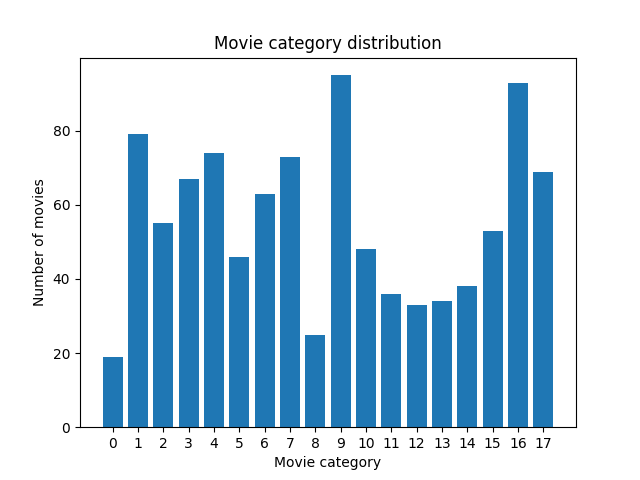
\includegraphics[width=\columnwidth]{figures/movie_category_distribution.png}
        \caption{Distribution of movie categories between 18 categories as in MovieLens dataset.}
        \label{fig:movie_category_distribution}
    \end{figure}

    The following \Cref{alg:algo1} shows our proposed procedure for creating additional features to run \textbf{BFM}

    \begin{algorithm}
        \SetKwInOut{Input}{input}
        Initialize missing matrix value with FM\\
        \For{$k = 0...K$} {
        Run SVD (rank=$k$)
        $k_{opt}=argmin_{k, k_{opt}}$RMSE(SVD(rank=$k$))
        }
            Movie embeddings= $\sqrt{\Sigma_{k_{opt}}}V_{k_{opt}}^T$\\
            Perform K-Means(movie embeddings)\\
            \For{$i = 0...numMovies$} {
            \For{$j = 0...numMovies$} {
            $D_{i,j} ^{Eucl} = \|embi - emb_j\|^2$
            }
                }
                \For{$i = 0...numMovies$} {
                \For{$j = 0...numMovies$} {
                $D_{i,j} ^{Mahal} = \sqrt{(emb_i-emb_j)^TCov^{-1}(emb_i-emb_j)}$
                }
                    }
                    \caption{Proposed solution for collaborative filtering}
                    \label{alg:algo1}
    \end{algorithm}

    With these additional user/item features, we append to our feature vector $\mathbf{x}_{ui}$ a dense vector of user similarities from user $u$ to every other user, or the item feature which is either the one-hot-encoded cluster of item $i$ or a dense vector of Euclidean/Mahalanobis distances from item $i$ to every other item.

    Finally, for our best model, we reformulated the task of predicting unobserved user/item pairs to a classification problem instead of a regression task where we calculate the expectation over the different class probabilities.

    \subsection{Neural Network based Approaches}

    \subsubsection{Neural Collaborative Filtering}
    Neural Collaborative Filtering approach as proposed by He et al. \cite{DBLP:journals/corr/abs-1708-05031}, tries to
    jointly learn user-item latent representations as well as the prediction depending on the interactions between
    different users and items. The network's inputs are indices of users and items. Firstly, an embedding layer maps
    each user and each item to its corresponding latent vector representation. Output of the embedding layers is then
    concatenated and passed on through fully connected feedforward layers with ReLU activation functions. Finally,
    output of the network represents the rating associated with the inputted user and item. Network is trained minimizing
    the mean squared error loss between the predicted and target rating. TODO: erase? Further, improvements would be
    implementing the network as a classification task between the movie rating rather then regressing the predicted rating.

    \subsubsection{Autoencoder}
    An autoencoder is a neural network that is trained to attempt to copy its input to its output.
    Internally, it has a hidden layer $\textbf{h} \in \mathbb{R}^k$ that describes a code used to represent the input.
    The network may be viewed as consisting of two parts: an encoder function $f: \mathbb{R} ^d \rightarrow \mathbb{R} ^k$ and a
    decoder that produces a reconstruction $g: \mathbb{R} ^k \rightarrow \mathbb{R} ^d$ \cite{Goodfellow-et-al-2016}.
    Autoencoders have proven to achieve good results in collaborative filtering \cite{inproceedings}.
    We examine the user-based autoencoder as opposed to item-based autoencoder which achieved a good score in \cite{inproceedings}.
    Both encoder and decoder consist of feedforward neural networks with ReLU activation functions.
    We train the model by minimizing the squared reconstruction loss.
    Important part of the implementation is the fact that inputs are partially observed and therefore we only update those weights that are associated with observed inputs during backpropagation.

    \subsubsection{AutoRec}
    Furthermore, we have run the AutoRec implementation \cite{inproceedings}, which achieved a state-of-the-art result.
    Compared to our autoencoder implementation AutoRec is item-based, uses the sigmoid activation function as the final non-linearity and adds regularization to the loss function.

    \subsubsection{Kernel Net}
    We add the MovieLens-1M state of the art model (on papers with code) as another baseline as the given problem description fares very similarly to ours.
    For this, we adapt the code from \cite{pmlr-v80-muller18a, kernelNetGithub} into our experiment framework.

    The high sparsity in recommender-system datasets leads to the need and resulting variety of possibilities for dimensionality reduction.
    Combined with the amount of parameters in neural networks this leads to large training times and possibly
    unexpected results on unseen data due to overfitting.

    Muller et al. make use of finite-support kernels to reparametrize weight matrices with low-dimensional vectors.
    This allows for the structured feature embedding of neural network weights based on the specific kernel function used and
    acts as regularization.
    As such, their item-based autoencoder is able to reduce complexity at inference time while improving performance compared to similar models.\cite{pmlr-v80-muller18a}

    \subsubsection{Iterative SVD}
    % maybe only have in results?
    % TODO: run from 1-10, 20-100


    \section{Results}
    We present our results in \Cref{tab:ablation}, noting the Root Mean Squared Error \textbf{(RMSE)} of our baselines and final model.
    Test scores refer to the public leaderboard ranking while validation scores refer to a 10\% holdout of our training data.
    Models without test scores were just added for completeness as the performance was not satisfactory or other models evaluated in the meantime performed better.
    Some other models may only show test scores if they were directly evaluated on the test data to eliminate
    fitting the model multiple times.

    All mentioned scores are after clipping the outputs to a range between 1 and 5 or, if stated otherwise, rounded to the closest quarter.
    However, using more sophisticated postprocessing techniques like rounding to integers or to quarters always resulted in worse performance.

    Looking at \Cref{fig:rank} we see that except for NMF, which achieves the lowest score with rank 24, the other models perform best with a rank of around 10.
    \begin{figure}
        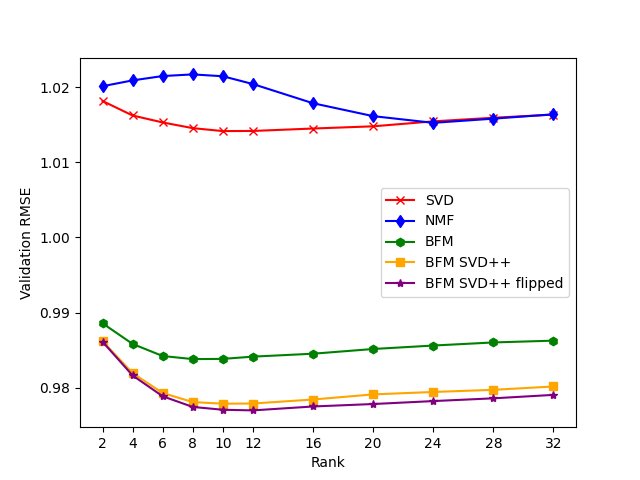
\includegraphics[width=\columnwidth]{figures/rank.png}
        \caption{Validation RMSE for different rank values.
        NMF performs best with a rank of 24 while the others do best with 8 - 12.}
        \label{fig:rank}
    \end{figure}


    Our first baseline, SVD, heavily depends on the initialization of unobserved values, achieving a test score of 0.9928 when replacing values with the item mean and only 1.0713 when using the overall mean (both rank 3).
    Due to this, we further experimented with using other models to predict the unobserved values.
    In \Cref{tab:ablation} SVD*10 stands for chaining 10 SVDs after another.
    With this we were able to get a test score of 0.9882 which is a large improvement.

    SVD + KernelNet first trains the KernelNet and then predicts the unobserved values so that they can be used as input for the SVD.
    This achieved a validation score of 0.9803 which increases to 0.9838 when chaining another 4 SVDs onto it.
    Utilizing our best BFM SVD++ f. (rank 12) in combination with 5 SVDs (rank 3) achieves the lowest SVD test score of 0.9846.

    Similar to the SVD, the NMF performs best (validation score of 0.9946) when replacing missing values with the item mean and then chaining 10 NMF models.

    We found that when both encoder and decoder in Autoencoder consist of one layer increasing the encoded dimension up to 500 makes
    the score better.
    Furthermore, we have examined the effect of compositionality.
    Using only two layers in encoder and decoder already performs better than any single layer Autoencoder getting a score of 1.0539 after 250 epochs.
    The AutoRec got an RMSE score of 1.0100 after only 5 epochs after which it gets worse.
    NCF after 10 epochs leads to a validation score of 1.0004, achieving its best of 0.9787 only after epoch 250.
    For our last Autoencoder, KernelNet, replacing the unobserved values with 0 surprisingly fared best.
    Using item mean like with SVDs leads to a much worse validation score of 1.0409 as opposed to 0.9831 when running it for 150 iterations.
    Similarly, running it for more than 150 iterations leads to a marginal decrease in score.

    From  \Cref{fig:validation} it is visible that overall the KernelNet performed best and Autoencoder made continuous progress, while AutoRec and NCF quickly started to overfit.

    \begin{figure}
        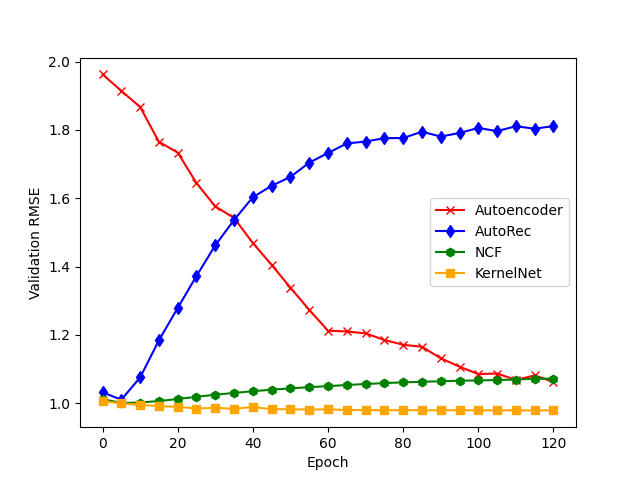
\includegraphics[width=\columnwidth]{figures/validation_plot.png}
        \caption{Validation RMSE for different epochs.
        AutoRec and NCF overfit after a few epochs while KernelNet and AutoEncoder show oppositve behaviour.}
        \label{fig:validation}
    \end{figure}


    Regarding our final baseline, we obtained similar overall results for BFM as stated in "On the Difficulty of Evaluating Baselines" \cite{rendle_difficulty_2019}.
    As can be seen in \Cref{tab:ablation}, BFM with implicit user and movie features performed best while standard BFM and BFM with only implicit user features performed worse.
    For our novelty of adding additional features for users and movies, we were not able to observe an improved.
    However, we noticed that the distance metrics performed worse when compared to the genre clustering hinting that with some fine-tuning of the cluster sizes, better results might be achievable.
    Compared to that, the introduction of the Jaccard index to resemble some connection between users performed similarly.
    An additional experiment that we conducted, was the idea to initialize SVD with the output of a BFM SVD++ flipped predictor and perform SVD iteratively multiple times.
    While this approach is unsurprisingly the best predictor for SVD due to its much better unobserved value initialization, it did not perform the overall best baseline.
    As a final approach, we reformulated the problem of predicting user/movie ratings from a regression problem into a classification one.
    This yielded a slight improvement which we could further decrease by using a lower rank approximation, namely 12 instead of 32.
    This might be due to the fact users tend to overall rate movies rather positive than negative for which we assume that this phenomenon can be better captured by formulating the problem of predicting user/movie ratings as a classification task.

    A general overview of low rank matrix approximation techniques can be observed in \Cref{fig:rank}.
    Here, we varied the amount of singular values to keep and reported the mean RMSE of a 3-fold cross validation.

    \subsection{Comparison to Baselines}
    % TODO: specifically compare best BFM model to the results of the best others, but have the details regarding the model in the description

    You compare your novel algorithm to \emph{at least two baseline
    algorithms}. For the baselines, you can use the implementations you
    developed as part of the programming assignments.



    \begin{table}
        \centering
        \resizebox{\columnwidth}{!}{
        \begin{tabular}{|| c | c | c | c | c ||}
            \hline
            \textbf{Model}       & \textbf{Params}                       & \textbf{ Init Missing } & \textbf{RMSE}$_{test}$ & \textbf{RMSE}$_{valid}$ \\
            \hline
            SVD                  & Rank 3                                & total mean              & 1.0713                 &                         \\
            SVD                  & Rank 3                                & user mean               & 1.0558                 &                         \\
            SVD                  & Rank 3                                & item mean               & 1.0138                 &                         \\
            SVD*4                & Rank 3                                & item mean               & 0.9928                 & 0.9893                  \\
            SVD*7                & Rank 3                                & item mean               & 0.9894                 &                         \\
            SVD*10               & Rank 3                                & item mean               & 0.9882                 & 0.9854                  \\
            SVD*10               & Rank 3, Round Quarters                & item mean               & 0.9907                 &                         \\
            SVD*10               & Rank 10                               & item mean               & 0.9941                 &                         \\
            SVD + KernelNet      & Rank 10 |150 Epochs                   & zero                    &                        & 0.9803                  \\
            5*SVD + KernelNet    & Rank 10 | 150 Epochs                  & zero                    &                        & 0.9838                  \\
            5*SVD + KernelNet    & Rank 3 | 150 Epochs                   & zero                    &                        & 0.9844                  \\
            5*SVD + BFM SVD++ f. & Rank 3 | Rank 12                      & /                       & 0.9846                 &                         \\
            \hline
            NMF                  & Rank 24                               & total mean              &                        & 1.0628                  \\
            NMF                  & Rank 24                               & user mean               &                        & 1.0497                  \\
            NMF                  & Rank 24                               & item mean               &                        & 1.0029                  \\
            NMF*10               & Rank 24                               & item mean               &                        & 0.9946                  \\
            \hline
            Autoencoder          & 50 Epochs                             & total mean              &                        & 1.3382                  \\
            Autoencoder          & 150 Epochs                            & total mean              &                        & 1.0757                  \\
            Autoencoder          & 250 Epochs                            & total mean              &                        & 1.0539                  \\
            \hline
            NCF                  & 50 Epochs                             & /                       &                        & 0.9820                  \\
            NCF                  & 150 Epochs                            & /                       &                        & 0.9789                  \\
            NCF                  & 250 Epochs                            & /                       &                        & 0.9787                  \\
            \hline
            AutoRec              & 5 Epochs                              & zero                    &                        & 1.0100                  \\
            AutoRec              & 25 Epochs                             & zero                    &                        & 1.3723                  \\
            AutoRec              & 50 Epochs                             & zero                    &                        & 1.6625                  \\
            \hline
            KernelNet            & 50 Epochs                             & zero                    & 1.0003                 & 0.9939                  \\
            KernelNet            & 150 Epochs                            & zero                    & 0.9860                 & 0.9831                  \\
            KernelNet            & 150 Epochs                            & item mean               &                        & 1.0409                  \\
            KernelNet            & 450 Epochs                            & zero                    & 0.9886                 &                         \\
            \hline
            BFM                  & Rank 12                               & /                       &                        & 0.9727                  \\
            BFM SVD++            & Rank 12                               & /                       &                        & 0.9664                  \\
            BFM SVD++ f.         & Rank 12                               & /                       &                        & 0.9655                  \\
            BFM SVD++ f.         & Jac. Sim., Rank 32                    & /                       & 0.9694                 &                         \\
            BFM SVD++ f.         & Improved Jacc. Sim., Rank 32          & /                       & 0.9974                 &                         \\
            BFM SVD++ f.         & Genre Clustering, Rank 32             & /                       & 0.9688                 &                         \\
            BFM SVD++ f.         & Mahalanobis Dist., Rank 32            & /                       & 1.0271                 &                         \\
            BFM SVD++ f.         & Euclidean Dist., Rank 32              & /                       & 0.9903                 &                         \\
            BFM SVD++ f.         & Ordered Prob., Rank 32                & /                       & \textbf{ 0.9657 }      &                         \\
            BFM SVD++ f.         & Ordered Prob., Round Quarter, Rank 32 & /                       & 0.9684                 &                         \\
            \hline
        \end{tabular}
        }
        \caption{We note Root Mean Squared Error (RMSE) on test and validation datasets to compare our baselines.
        Arithmetic in models such as $x * 4$ or $x + y$ refers to the iterative chaining of multiple models for the initialization of missing values.
        }
        \label{tab:ablation}
    \end{table}


    \begin{figure}
        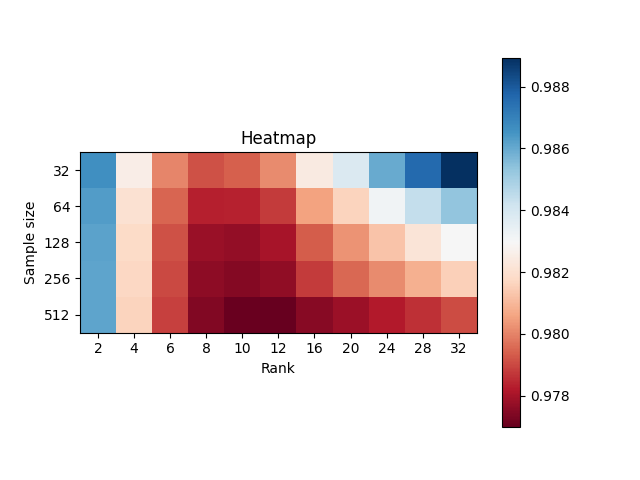
\includegraphics[width=\columnwidth]{figures/heatmap.png}
        \caption{Validation RMSE for different values of sample size and rank produced by grid search on our best BFM model.
        Ranks of 8 - 12 in combination with higher sample sizes perform best.}
        \label{fig:Heatmap}
    \end{figure}


    \section{Discussion}
    As stated in the previous section, the introduction of additional hand-crafted features for users and movies did not yield any significant improvement.
    We assume that this is mainly based on the statistical learning theory fact that one cannot gain additional information out of existing data.
    Although, the genre clustering as well as the standard Jaccard index did not perform much worse than the standard baselines, we conclude that hand-crafting features for collaborative filtering is not a direction worth exploring.

    % TODO primarily BMF

    %TODO importance of shuffeling
    %add info that we trained on whole dataset


    \section{Summary}

    Organize the results section based on the sequence of table and
    figures you include. Prepare the tables and figures as soon as all
    the data are analyzed and arrange them in the sequence that best
    presents your findings in a logical way. A good strategy is to note,
    on a draft of each table or figure, the one or two key results you
    want to address in the text portion of the results.
    The information from the figures is
    summarized in Table.




    \balance
    \bibliographystyle{IEEEtran}
    \bibliography{bibliography}
\end{document}
